\chapter{Implementierung}\label{chap_impl}
Die Implementierung der \emph{Explorationskomponente} besteht aus drei Teilen, die jeweils als separates Java-Projekt umgesetzt wurden. Im weiteren Verlauf werden diese Java-Projekte als \Gls{Modul}e bezeichnet.In Abbildung \ref{cd_arch} ist die Architektur der \emph{Explorationskomponente} mit diesen drei \Gls{Modul}en aufgeführt.
\begin{figure}[h!]
\centering
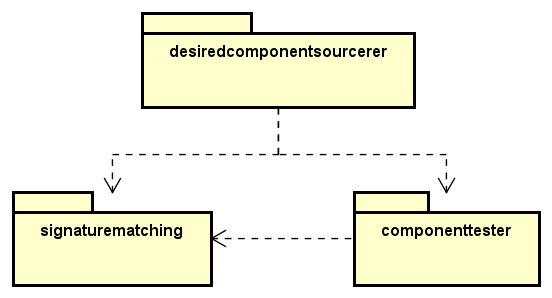
\includegraphics[scale=0.8]{cd_arch.png}
\caption{Architektur}
\label{cd_arch}
\end{figure}
\noindent
\\
Im weiteren Verlauf dieses Kapitels werden die \Gls{Modul}e einzeln beschrieben . Das \Gls{Modul} \emph{DesiredComponentSourcerer} ist dabei von den \Gls{Modul}en \emph{ComponentTester} und \emph{SignatureMatching} abhängig, während das \Gls{Modul} \emph{ComponentTester} lediglich vom \Gls{Modul} \emph{SignatureMatching} abhängig ist.
\\\\
Darüber hinaus, werden folgende externe Bibliotheken verwendet:
\begin{itemize}
%\item easymock 3.0 \cite{easymock}
\item cglib 3.3.0 \cite{cglib}
\item objenesis 3.1 \cite{objenesis}
\item junit 4.13.0 \cite{junit}
\end{itemize}
Auf die konkrete Verwendung der externen Bibliotheken wird in den detaillierteren Beschreibungen der einzelnen \Gls{Modul}e eingegangen.
\section{Modul: SignatureMatching}\label{impl_sigma}
\begin{figure}[h!]
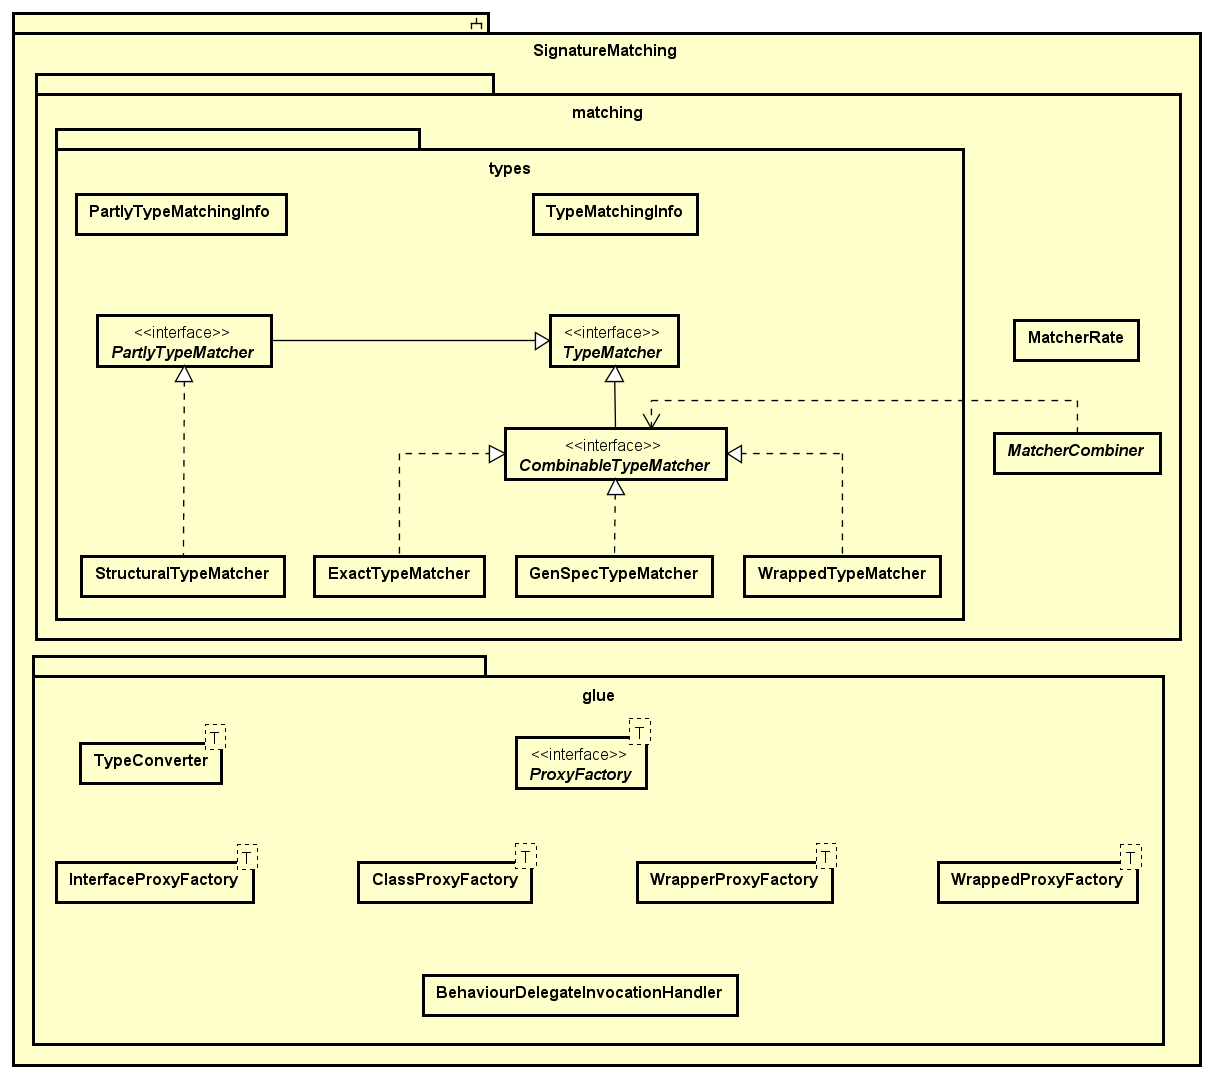
\includegraphics[scale=0.5]{cd_SigMa.png}
\caption{Modul: SignatureMatching}
\label{fig_cdSigMa}
\end{figure}
\noindent
In diesem \Gls{Modul} befinden sich zum einen die Implementierungen der Matcher, die in Abschnitt \ref{sec_matcher} formal beschrieben wurden und zum anderen die Implementierung der Generatoren für die \emph{Proxies}. In Abbildung \ref{fig_cdSigMa} sind die wichtigsten Klassen und \Gls{Interface}s dieses \Gls{Modul}s mit ihren Abhängigkeiten zueinander aufgeführt. Die Matcher befinden sich dabei im Package \texttt{matching} und die Generatoren für die \emph{Proxies} in Form der Implementierungen des \Gls{Interface}s $\texttt{ProxyFactory}$ im Package \texttt{glue}.
\\\\
Die in Abschnitt \ref{sec_matcher} beschriebenen Matcher und Generatoren wurden teilweise in einer Klasse zusammengefasst. Tabelle \ref{tab_matcher2impl} zeigt die Zuordnung von Matchern zu den jeweiligen Klassen, die die Implementierung dieser darstellen (Spalte: Matcher-Implementierung). Zudem sind in der Tabelle \ref{tab_matcher2impl} auch die Klassen ausgewiesen, die die Implementierung des Generators für den Proxy, der auf Basis des Matchers Anwendung findet, darstellen (Spalte: Generator-Implementierung).
\begin{table}[h!]
\centering
\begin{tabular}{|l|l|l|}
\hline
\hline
\textbf{Matcher} & \textbf{Matcher-Implementierung} & \textbf{Generator-Implementierung}\\
\hline
ExactTypeMatcher & $\texttt{ExactTypeMatcher}$ &  \\
\hline
GenTypeMatcher & $\texttt{GenSpecTypeMatcher}$ & \\
\hline
SpecTypeMatcher & $\texttt{GenSpecTypeMatcher}$ & $\texttt{SubProxyFactory}$\\
\hline
ContentTypeMatcher & $\texttt{ContainerTypeMatcher}$ & $\texttt{ContentProxyFactory}$\\
\hline
ContainerTypeMatcher & $\texttt{ContainerTypeMatcher}$ & $\texttt{ContainerProxyFactory}$\\
\hline
StructuralTypeMatcher & $\texttt{StructuralTypeMatcher}$ & $\texttt{StructProxyFactory}$\\
\hline
\hline
\end{tabular}
\caption{Zuordnung der Matcher zu den Matcher- und Generator-Implementierungen}
\end{table}\label{tab_matcher2impl}
\noindent
\\\\
Die Klasse $\texttt{StructuralTypeMatcher}$ nimmt bei den Matcher-Klassen eine Sonderstellung ein. Dies ist daran zu erkennen, dass dieser nicht das \Gls{Interface} $\texttt{TypeMatcher}$ implementiert. Das liegt daran, dass es sich bei diesem Matcher um den Einstiegspunkt der \emph{strukturellen Evaluation} handelt. Analog zum \emph{StructuralTypeMatcher} aus Abschnitt \ref{sec_matcher} wird in der Klasse $\texttt{StructuralTypeMatcher}$ auf die anderen Matcher bzw. Matcher-Klassen zugegriffen, was in Abbildung \ref{fig_cdSigMa} durch die Aggregation zwischen der Klasse $\texttt{StructuralTypeMatcher}$ und dem \Gls{Interface} $\texttt{TypeMatcher}$ angedeutet werden soll.
\\\\
Die übrigen Matcher-Klassen implementieren das \Gls{Interface} $\texttt{TypeMatcher}$ und können über die Methode $\texttt{combine}$ aus der Klasse $\texttt{MatcherCombinator}$ miteinander kombiniert werden\footnote{Ein Beispiel für die Kombination von Matchern ist im Anhang \ref{app_matchercombination} zu finden.}. 
\\\\
So kann eine Kombination mehrerer $\texttt{TypeMatcher}$, die wiederum von Typ $\texttt{TypeMatcher}$ ist, in der Klasse $\texttt{StructuralTypeMatcher}$ verwendet werden. Die konkrete $\texttt{TypeMatcher}$-\linebreak Kombination, die im $\texttt{StructuralTypeMatcher}$ instanziiert wird, orientiert sich an den \linebreak Ausführungen in Abschnitt \ref{sec_matcher} (siehe auch Anhang \ref{app_matchercombination}). Es ist aber zu erwähnen, dass die Verwendung weiterer Matcher, die in dieser Arbeit nicht definiert wurden, denkbar ist. Eine solche Erweiterung ließe sich leicht in dieses \Gls{Modul} über die Implementierung des \Gls{Interface}s $\texttt{TypeMatcher}$ und die Verwendung der Klasse $\texttt{MatcherCombiner}$ vornehmen.
\\\\
Alle Matcher-Implementierungen bieten die Möglichkeit, zu ermitteln, ob ein Matching zwischen zwei Typen besteht (siehe Klassendiagramme in Abbildungen \ref{fig_cdMatchingInfo} und \ref{fig_cdSingleMatchingInfo}). Dies erfolgt jeweils über die Methode $\texttt{matchesType}$. Über die Methode $\texttt{calculateMatchingInfos}$ werden die Informationen bzgl. der Methodendelegationen zwischen den beiden gematchten Typen ermittelt. Diese Informationen werden in einem Objekt der Klasse $\texttt{SingleMatchingInfo}$ bzw. $\texttt{MatchingInfo}$ zusammengetragen, welche in Abbildung \ref{fig_cdMatchingInfo} und \ref{fig_cdSingleMatchingInfo} detailliert dargestellt werden.
\begin{figure}[h!]
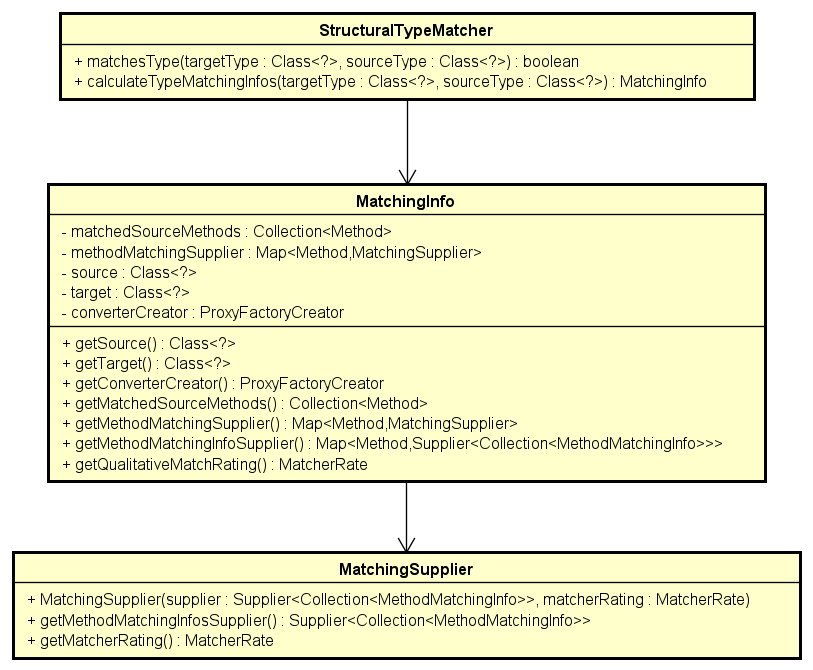
\includegraphics[scale=0.8]{cd_matchinginfo.png}
\caption{Klassendiagramm: $\texttt{StructuralTypeMatcher}$ und $\texttt{MatchingInfos}$}
\label{fig_cdMatchingInfo}
\end{figure}
\begin{figure}[h!]
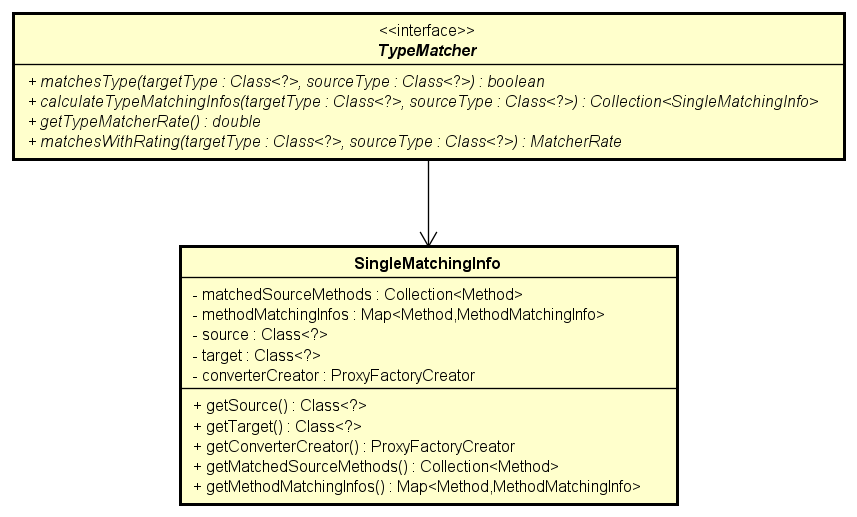
\includegraphics[scale=0.7]{cd_singlematchinginfo.png}
\caption{Klassendiagramm: $\texttt{TypeMatcher}$ und $\texttt{SingleMatchingInfo}$}
\label{fig_cdSingleMatchingInfo}
\end{figure}
\noindent
\\\\
Diese beiden Klassen unterscheiden sich lediglich bzgl. des Attributs in dem die Delegationsmethoden hinterlegt sind. Dabei handelt es sich auf Seiten der $\texttt{SingleMatchingInfo}$ um das Attribut $\texttt{methodMatchingInfos}$ und auf Seiten der $\texttt{MatchingInfo}$ um das Attribut \linebreak$\texttt{methodMatchingSupplier}$. 
\\\\
Während ein Objekt der Klasse $\texttt{MatchingInfo}$ mehrere \emph{Delegationsmethoden} zu einer \emph{aufgerufenen Methoden} enthalten kann, darf ein Objekt der Klasse $\texttt{SingleMatchingInfo}$ lediglich eine \emph{Delegationsmethode} zu einer \emph{aufgerufenen Methode} enthalten (vgl. auch Abschnitt \ref{sec_matcher}). Zusätzlich zu erwähnen ist, dass die Informationen über die \emph{Delegationsmethoden} aus einer $\texttt{MatchingInfo}$ über einen $\texttt{MethodSupplier}$ überliefert werden.
\\\\
Eine Instanz der Klasse $\texttt{MethodSupplier}$ enthält zum einen ein $\texttt{MatcherRating}$ welches Informationen bzgl. des in Abschnitt \ref{sec_lmf} beschriebenen \emph{Matcherratings} beinhaltet. Zum anderen werden im Attribut $\texttt{methodMatchingInfo}$ in einem Objekt der Klasse $\texttt{MethodMatchingInfo}$ (siehe Abbildung \ref{cd_methodMatchingInfo}) die Informationen bzgl. der Delegation der \emph{aufgerufenen Methode} an die \emph{Delegationsmethode} hinterlegt. 
\\\\
Bezüglich der Klasse $\texttt{SingleMatchingInfo}$ ist noch das Attribut $\texttt{proxyFactoryCreator}$ zu beschreiben. Darin werden Informationen bzgl. der strukturellen Verbindung zwischen den gematchten Typen gehalten. 
\\\\
Für den \emph{ExactTypeMatcher}, den \emph{GenTypeMatcher} und den \emph{SpecTypeMatcher} wird dabei ein $\texttt{ProxyFactoryCreator}$ erzeugt, das in der Lage ist, eine $\texttt{ProxyFactory}$ für Typen zu erzeugen, die in einer nominalen Beziehung \footnote{Identität, Generalisierung, Spezialisierung} stehen. 
\\\\
Für den \emph{ContentTypeMatcher} und den \emph{ContainedTypeMatcher} hingegen, wird ein Objekt vom Typ $\texttt{ProxyFactoryCreator}$ erzeugt, der in der Lage ist, eine $\texttt{ProxyFactory}$ für Typen zu erzeugen, bei denen der eine Typ ein Attribut vom Typ des anderen enthält (vgl. mit Tabelle \ref{tab_matcher2impl}). Die erzeugten Objekte vom Typ $\texttt{ProxyFactory}$ werden bei der Generierung der \emph{Proxies} unter der Zuhilfenahme der Bibliotheken \emph{cglib} und \emph{objenesis} verwendet\footnote{Diese beiden Frameworks wurden verwendet, da die Erzeugung der \emph{Proxies} mit ihnen komfortabler ist, als mit den Mitteln die das JKD zur Verfügung stellt. Dies gilt insbesondere für die Erzeugung von \emph{Proxies} für Klassen, die mit dem Schlüsselwort $\texttt{final}$ versehen sind. (vgl. \cite{objenesis}, \cite{cglib})}.
\\\\
Der $\texttt{ProxyFactoryCreator}$ stellt damit eines der Bindeglieder zwischen der Package \texttt{matching} und dem Package \texttt{glue} innerhalb dieses \Gls{Modul}s her. Das zweite \Gls{artefakt}, welches als Bindeglied fungiert, ist die oben bereits erwähnte Klasse $\texttt{MethodMatchingInfo}$, deren Aufbau dem Klassendiagramm aus Abbildung \ref{cd_methodMatchingInfo} zu entnehmen ist.
\begin{figure}[h!]
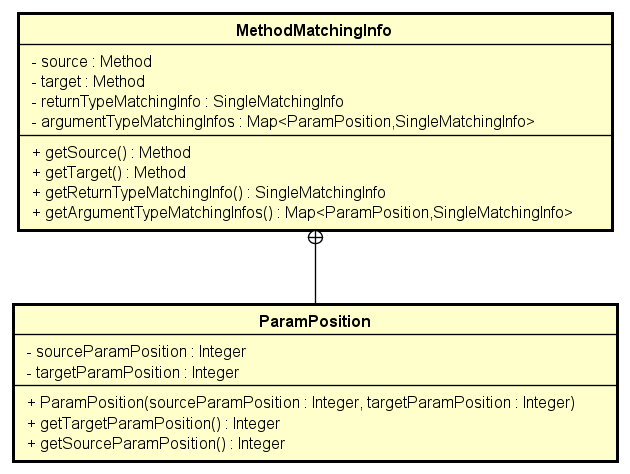
\includegraphics[scale=1.0]{cd_methodmatchinginfo.png}
\caption{Klassendiagramm: $\texttt{MethodMatchingInfo}$}
\label{cd_methodMatchingInfo}
\end{figure}
\noindent
\\\\
Ein Objekt der Klasse $\texttt{MethodMatchingInfo}$ enthält in den Attributen $\texttt{source}$ und $\texttt{target}$ je eine Methode. Dabei ist im Attribut $\texttt{source}$ die \emph{aufgerufene Methode} der \emph{Methoden-Delegation} und im Attribut $\texttt{target}$ die \emph{Delegationsmethode} hinterlegt. Darüber hinaus wird im Attribut $\texttt{returnTypeMatchingInfo}$ ein Objekt der Klasse $\texttt{SingleMatchingInfo}$ gehalten, welches alle notwendigen Informationen für das Erzeugen eines \emph{Proxies} des Rückgabetyps der \emph{aufgerufenen Methode} aus dem Rückgabetyp der \emph{Delegationsmethode} enthält.
\\\\
Analog dazu wird im Attribut $\texttt{argumentTypeMatchingInfos}$ eine Map, bestehend aus weiteren Objekten der Klasse $\texttt{SingleMatchingInfo}$ und jeweils einem Objekt der Klasse $\texttt{ParamPosition}$, gehalten. Diese Map enthält alle notwendigen Information für das Erzeugen eines \emph{Proxies} für die Parametertypen der \emph{Delegationsmethoden} aus den Parametertypen der \emph{aufgerufenen Methode}, sowie der Anpassung der Übergabeposition bei der Delegation der \emph{aufgerufenen Methode} (siehe auch Abschnitt \ref{sec:proxygram}).
\\\\
Um die \emph{Methoden-Delegationen} zu koordinieren, wird bei der Erzeugung des \emph{Proxies} in der jeweiligen $\texttt{ProxyFactory}$ für das \emph{Proxy}-Objekt ein $\texttt{InvocationHandler}$ instanziiert (vgl. \cite{invocationhandler}). Dieses \Gls{Interface} wird im Sub-Package \texttt{glue.delegation} durch die Klasse \linebreak$\texttt{BehaviourDelegateInvocationHandler}$ implementiert, in der letztendlich die Koordination der \emph{Methoden-Delegationen} auf Basis der jeweiligen $\texttt{MethodMatchingInfo}$ spezifiziert ist.
\\\\
Um einen \emph{Proxy} basierend auf dem Matching zweier Typen zu erzeugen, steht die Klasse $\texttt{TypeConverter}$ zur Verfügung (siehe Abbildung \ref{cd_typeconverter}). Die Zugriffe innerhalb des Packages \texttt{glue} als auch die Zugriffe von außerhalb verlangen jeweils ein Objekt der Klasse $\texttt{ConvertableBundle}$. Diese Klasse beschreibt eine Kombination mehrerer Objekte vom Typ $\texttt{ConvertableComponent}$, die als \emph{Target-Typen} des zu erzeugenden Proxy-Objektes fungieren sollen. Ein Objekt der Klasse $\texttt{ConvertableComponent}$ enthält eine Liste von Objekten vom Typ $\texttt{SingleMatchingInfo}$, die wie bereits erwähnt beschreiben, am welche Methode die Delegation erfolgen soll. Das Objekt im Attribut $\texttt{convertableObject}$ der $\texttt{ModuleMatchingInfo}$ beinhaltet das Objekt, auf dem die \emph{Delegationsmethode} aufgerufen werden soll.
\begin{figure}[h!]
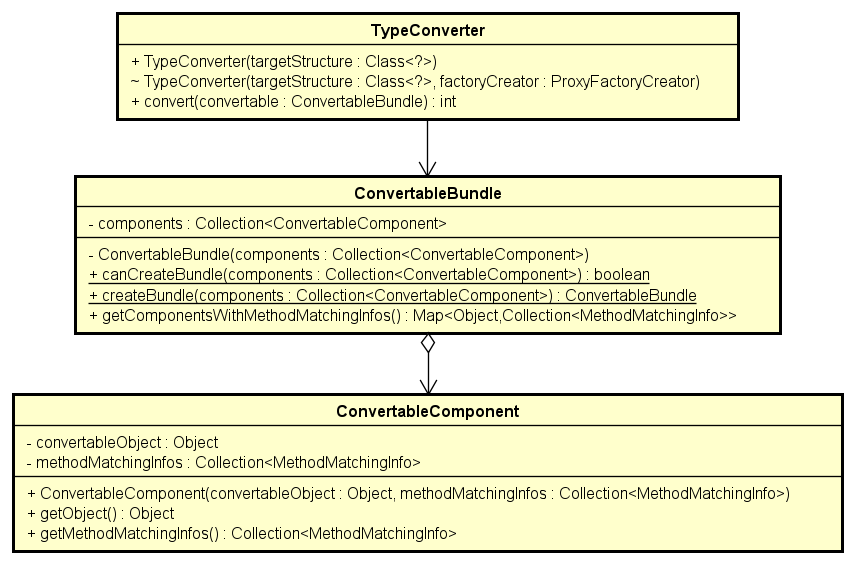
\includegraphics[scale=0.7]{cd_typeconverter.png}
\caption{Klassendiagramm: $\texttt{TypeConverter}$}
\label{cd_typeconverter}
\end{figure}

\section{Modul: ComponentTester}\label{sec_Impl_CT}
Dieses \Gls{Modul} ist für die Ausführung der vordefinierten Tests zuständig. Darüber hinaus bietet es die Möglichkeit, die vordefinierten Tests mit den \Gls{Interface}s, die den jeweiligen \emph{required Typ} darstellen, zu verbinden. Dabei sei davon auszugehen, dass ein \emph{required Typ} $R$ in Form eines \Gls{Interface}s existiert. Um die Tests für $R$ zu definieren, können eine oder mehrere Testklassen implementiert werden.
\\\\
Die Testklassen werden dabei in dem \Gls{Interface} $R$ über das Attribut $\texttt{testClasses}$ der Annotation $\texttt{RequiredTypeTestReference}$ angegeben (siehe Abbildung \ref{fig_cdCompTester} Package: \texttt{api}). Ein Beispiel für die Deklaration eines solchen \Gls{Interface}s und den dazugehörigen Testklassen ist im Anhang \ref{app_interfacesAndTests} zu finden.
\\\\
Damit die Testmethoden in den Testklassen die in Abschnitt \ref{sec_testanforderungen} beschriebenen Eigenschaften aufweisen und durch das \emph{ComponentTester}-\Gls{Modul} ausfindig gemacht werden können, stehen mehrere \Gls{artefakt}e in dem \texttt{api}- und dem \texttt{spi}-Package des \emph{ComponentTester}-\Gls{Modul}s bereit (siehe Abbildung \ref{fig_cdCompTester}).
\begin{figure}[H]
\centering
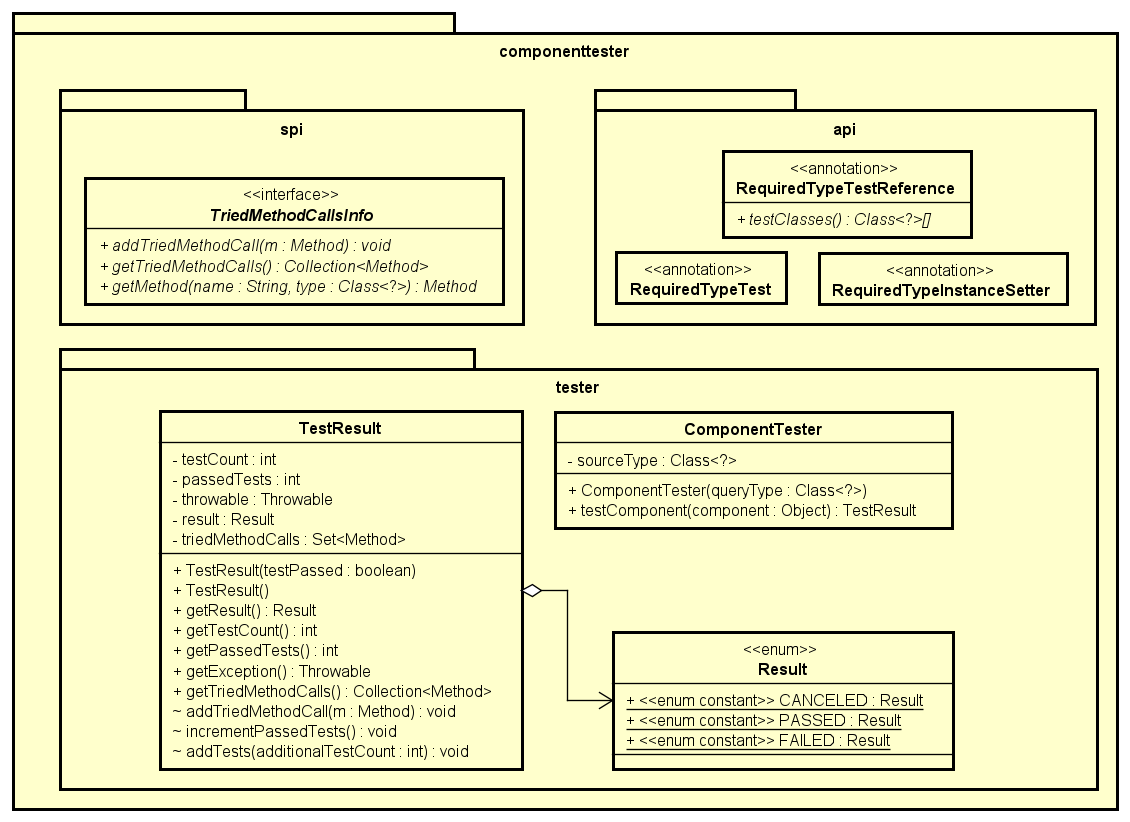
\includegraphics[scale=0.6]{pics/cd_ComponentTester.png}
\caption{Modul: ComponentTester}
\label{fig_cdCompTester}
\end{figure}
\noindent
So muss jede Testklasse eine Methode bereitstellen, über die ein Objekt vom Typ $R$ in die Instanz der Testklasse injiziert werden kann.\footnote{auch genannt: Setter-Injection (vgl. \cite{setterinjection})} Diese Methode wird von dem \emph{ComponentTester}-\Gls{Modul} über die Annotation $\texttt{RequiredTypeInstanceSetter}$ gefunden. Von daher muss die Methode mit eben dieser Annotation markiert werden.
\\\\
Die Testmethoden müssen von der Sichtbarkeit her öffentlich ($\texttt{public}$) sein. Weiterhin dürfen die Testmethoden keine Parameter erwarten und müssen mit der Annotation $\texttt{RequiredTypeTest}$ markiert sein. Die Erwartungen innerhalb der Testmethoden müssen über die in JUnit 4 zur Verfügung stehenden Methoden aus der Klasse $\texttt{Assert}$ (siehe auch \cite{junit_api}) deklariert werden. Testdaten, die für alle Testmethoden innerhalb einer Testklasse zur Verfügung stehen sollen, können über Methoden bereitgestellt werden, die mit den durch die JUnit 4 Bibliothek bereitgestellten Annotationen $\texttt{Before}$ und $\texttt{After}$ (vgl. \cite{junit_api}) markiert wurden.
\\\\
Um die Reihenfolge der versuchten Aufrufe der Methoden, die von $R$ angeboten werden, zu verwalten\footnote{Das ist für die \Gls{Heuristik} \emph{BL\_NMC} notwendig. (vgl. auch Abschnitt \ref{sec_bl_nmc})}, muss die Testklasse das \Gls{Interface} $\texttt{TriedMethodCallsInfo}$ implementieren (siehe Abbildung \ref{fig_cdCompTester} Package: \texttt{spi}). Dadurch wird die Implementierung der Methoden $\texttt{addTriedMethodCall}$ und $\texttt{getTriedMethodCalls}$ erzwungen. Die Methode $\texttt{getMethod}$ kann mit der Defaultimplementierung übernommen werden, sofern die in $R$ deklarierten Methoden über den Namen identifiziert werden können.
\\\\
Die Implementierung der Methoden $\texttt{addTriedMethodCall}$ und $\texttt{getTriedMethodCalls}$ hat so zu erfolgen, dass bei einem Aufruf der Methode $\texttt{addTriedMethodCall}$ der übergebene Parameter an eine Liste angefügt wird. Der Aufruf der Methode $\texttt{getTriedMethodCalls}$ liefert eben diese Liste als Rückgabewert. Weiterhin ist sicherzustellen, dass vor dem Aufruf einer Methode $m$ aus $R$ die Methode $\texttt{addTriedMethodCall}$ mit $m$ als Parameter aufgerufen wird. Im Anhang \ref{app_interfacesAndTests} sind mehrere Beispiele für die korrekte Implementierung von Testklassen zu finden\footnote{siehe Listings \ref{lst_testklassen_tei1} - \ref{lst_testklassen_tei7}}.
\\\\
Die Durchführung der Tests, die für $R$ definiert wurde, wird über eine Instanz der Klasse $\texttt{ComponentTester}$ gestartet (siehe Abbildung \ref{fig_cdCompTester} Package: \texttt{tester}). In Abhängigkeit der in $R$ deklarierten Testklassen werden alle darin befindlichen Testmethoden mit einem \emph{Proxy} für $R$ durchgeführt, bis einer dieser Testfälle fehlschlägt. Der Aufrufer der Testdurchführung erhält dabei ein Objekt der Klasse $\texttt{TestResult}$ zurück (siehe Abbildung \ref{fig_cdCompTester}). In diesem Objekt sind die für die Auswertung des Testergebnisses relevanten Informationen vorhanden, auf die die \Gls{Heuristik}en \emph{PTTF} (siehe Abschnitt \ref{sec_pttf}) und \emph{BL\_NMC} (siehe Abschnitt \ref{sec_bl_nmc}) angewiesen sind.
\section{Modul: DesiredComponentSourcerer}\label{sec_impl_descos}
In diesem \Gls{Modul} befindet sich die Implementierung für den Einsteigspunkt des \emph{Explorationsprozesses}. Zum Starten des \emph{Explorationsprozesses} für ein \emph{required Typ} $R$ in Form eines \Gls{Interface}s muss zuerst eine Instanz der Klasse $\texttt{DesiredComponentFinder}$ erzeugt werden (genannt: \emph{Finder}). Dies erfolgt über einen Konstruktor, der ein Objekt der Klasse \linebreak$\texttt{DesiredComponentFinderConfig}$ (genannt: \emph{Konfig}) erwartet (siehe Abbildung \ref{cd_descos}). 
\begin{figure}[h!]
\centering
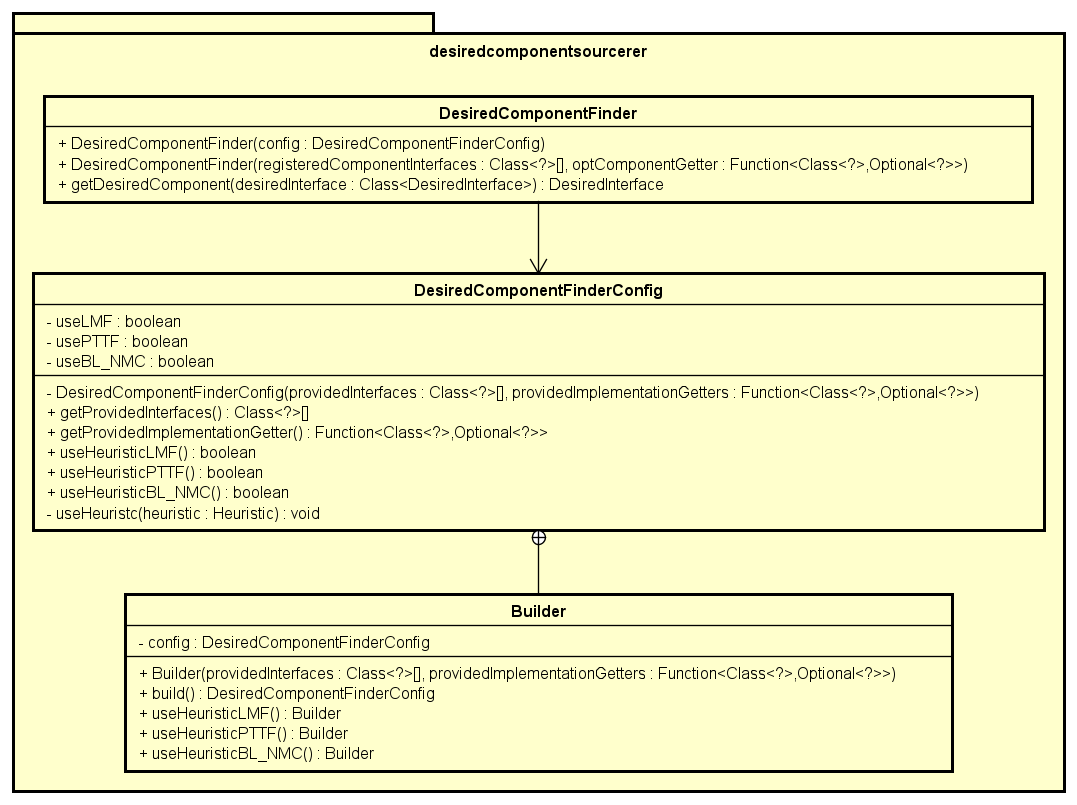
\includegraphics[scale=0.5]{cd_descos.png}
\caption{Modul: DesiredComponentSourcerer}
\label{cd_descos}
\end{figure}
\noindent
\\\\
Die Instanziierung einer solchen \emph{Konfig} erfolgt über die Klasse $\texttt{Builder}$\footnote{Builder-Pattern (siehe auch \cite{patterns})}. Dabei müssen zum einen alle  \emph{provided Typen} in Form einer Liste von \Gls{Interface}s angegeben werden\footnote{In Bezug auf \emph{EJBs} sind hier also alle \emph{EJB}-\Gls{Interface}s anzugeben}. Zum anderen wird eine Funktion ($\texttt{java.util.Function}$) gefordert, über die die Implementierungen jener \Gls{Interface}s ermittelt werden können.
\\\\
Zum Zweck der gezielten Evaluation der \Gls{Heuristik}en im folgenden Kapitel kann über die \emph{Konfig} gesteuert werden, welche der in Abschnitt \ref{sec_heuristics} beschriebenen \Gls{Heuristik}en während des \emph{Explorationsprozesses} verwendet werden sollen. Dies erfolgt über die in Abbildung \ref{cd_descos} ersichtlichen Methoden mit den Präfix $\texttt{useHeuristic}$.
\\\\
Nachdem der \emph{Finder} erzeugt wurde, kann der \emph{Explorationsprozess} über die Methode \linebreak$\texttt{getDesiredComponent}$ mit der Übergabe des \Gls{Interface}s für den \emph{required Typ} $R$ als Parameter gestartet werden. Im Anschluss wird die \emph{strukturelle Evaluation} für alle \emph{provided Typen}  durchgeführt. Hierzu wird ein Objekt vom $\texttt{StructuralTypeMatcher}$ aus dem \emph{SignatureMatching}-\Gls{Modul} verwendet\footnote{Dieses Objekt wird beim Instanziieren des \emph{Finders} erzeugt (siehe auch Anhang \ref{app_matchercombination}: Listing \ref{lst_matchermanager}).} und versucht die \emph{provided Typen} mit dem \emph{required Typ} zu matchen.
\\\\
Auf formaler Ebene gleicht dieser Schritt der Ausführung der Funktion $\mathit{cover(R,L)}$, wobei die in $L$ befindlichen \emph{provided Typen} auf die Typen, die dem \emph{Finder} bei der Instanziierung übergebenen wurden, beschränkt sind.
\\\\
Nach der \emph{strukturellen Evaluation}, wird gemäß Abschnitt \ref{sec_semEval} die \emph{semantische Evaluation} durchgeführt. Dabei werden zuerst die \emph{Proxies} aus den Kombinationen der gematchten \emph{provided Typen}\footnote{Diese Kombinationen sind auf formaler Ebene Äquivalent zu den Elementen der Mengen aus $\mathit{cover(R,L)}$.} erzeugt, welche im Anschluss hinsichtlich der vordefinierten Tests bzgl. des \emph{required Typs} $R$ geprüft werden. Dabei werden die \Gls{Heuristik}en, die in der \emph{Konfig} hinterlegt wurden, angewendet. Sofern während des \emph{Explorationsprozesses} ein \emph{Proxy} erfolgreich getestet wurde, wird dieser als Ergebnis des Aufrufs der Methode $\texttt{getDesiredComponent}$ zurückgegeben. Falls kein \emph{Proxy} die Tests besteht, wird $\texttt{null}$ zurückgegeben.
